\chapter{Objetivos} 
%----------------------------------------------------------------------------------------
%	SECTION 1
%----------------------------------------------------------------------------------------
Una vez  presentado el contexto en el que se basa este trabajo, pasamos a definir los objetivos que se cubren en el TFG.

El objetivo principal es desarrollar un conjunto de practicas basadas en tecnologías web que sirva como modelo a los alumnos de la asignatura de LTAW. Cada una de estas practicas se trata como un subobjetivo en la siguiente lista.
\begin{enumerate}
\item  Crear un juego en la web basado en tecnologías del cliente.
\item Crear un juego multijugador basado en tecnologías de comunicación bidireccional en tiempo real.
\item Crear un sitio Web de eventos y cantantes basada en tecnologías de servidor con manejo de base de datos.
\item Crear una aplicación de Videoconferencia Peer-to-Peer entre navegadores basada en tecnologías de comunicación audiovisual.
\end{enumerate}
%----------------------------------------------------------------------------------------
%	SECTION 2
%----------------------------------------------------------------------------------------
\section{Metodología}
La realización de todo proyecto necesita una metodología a seguir con el que se planifica las tareas necesarias para llegar a nuestro objetivo. Por ello se ha seleccionado el modelo de desarrollo en espiral, figura \ref{fig:espiral},que se aplica habitualmente en ingeniería de software.
\\Este modelo define una serie de ciclos que se repiten continuamente hasta finalizar el proyecto, dividiéndolo en subtareas mas sencillas en las que se establece un punto de control al final de cada una para evaluar el resultado y establecer nuevas tareas.

Durante el tiempo que ha durado el proyecto se acordaron reuniones semanales con el tutor de forma presenciales o por Video-Conferencia en las que se revisaba los objetivos semanas y se definían los nuevos objetivos.

Los avances mas relevantes se añadían a la mediawiki \cite{Mediawiki} de JdeRobot y a través de repositorio de GitHub \cite{Repositorio} guardábamos el código.
\section{Plan de trabajo}
Para finalizar este capitulo explicamos las distintas partes en las que se ha divido el plan del proyecto.
\begin{enumerate}
\item \textbf{Aprendizaje de tecnologías web:} Estudiar y conocer distintas tecnologías web del servidor, cliente, BBDD y tecnologías de intercambio de información entre el cliente y el servidor.
\item \textbf{Selección de practicas:} Con los conocimientos adquiridos realizamos una propuesta que se ajuste a los requisitos marcados.
\item \textbf{Desarrollo de practicas:} El diseño y desarrollo de cada practica ha sido de forma incremental,es decir,se ha buscado obtener la funcionalidad exigida en cada una para luego centrarnos en dar una apariencia mas atractiva.
\item \textbf{Pruebas:} Cada una de las practicas han sido ejecutadas en distintos navegadores para evaluar su funcionalidad.
\end{enumerate}
\begin{figure}[!h]
\centering
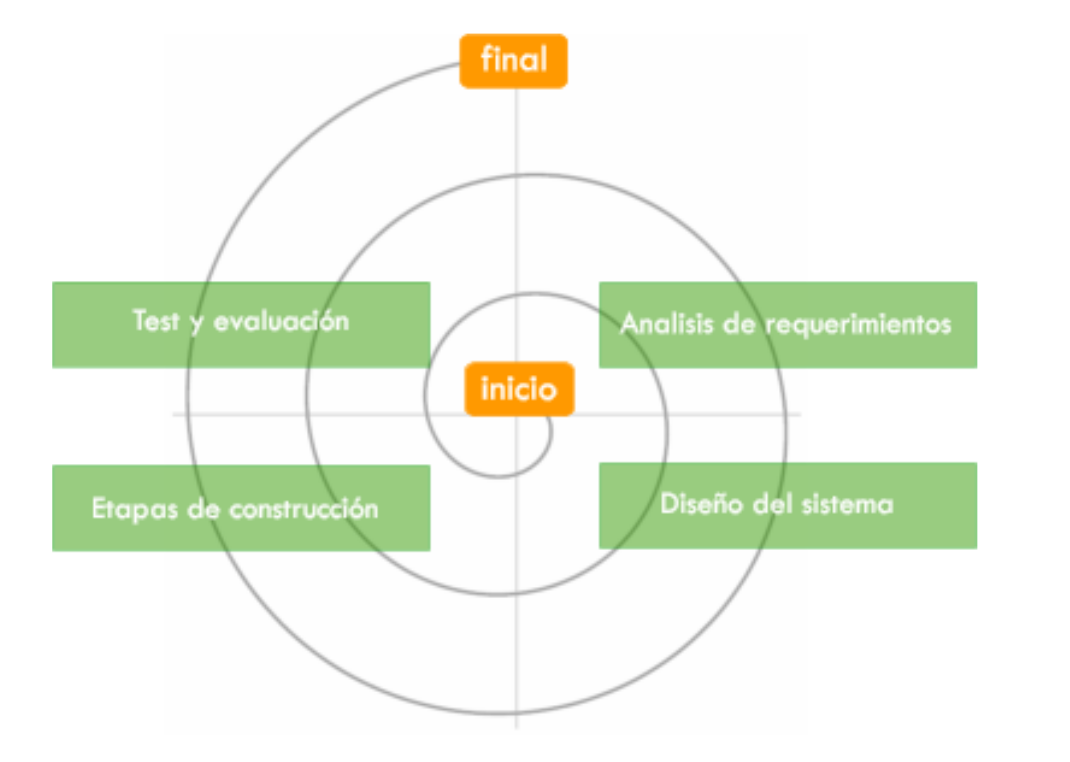
\includegraphics[width=0.8\linewidth]{Figures/espiral}
\decoRule
\caption[Metodología en espiral]{Metodología en espiral.}
\label{fig:espiral}
\end{figure}
